\begin{frame}
\frametitle{Scope - exciting and mundane sea level}

- Desktop study
- Operational system and data wrangling

\begin{figure}[h]\centering
  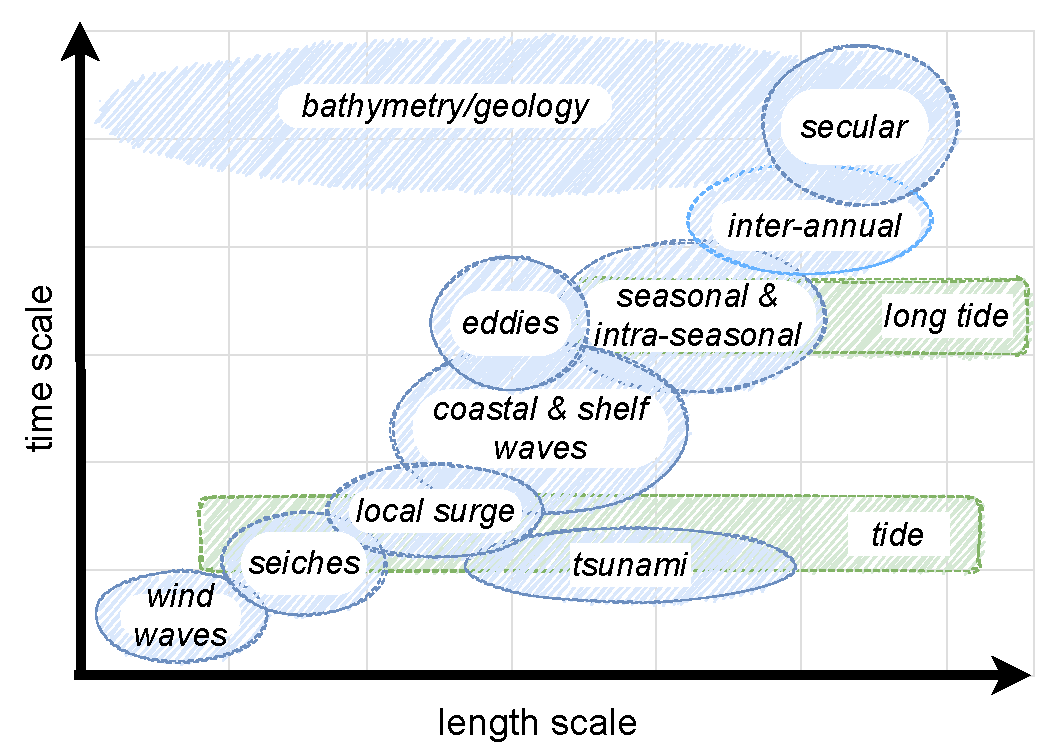
\includegraphics[width=130mm]{figures/diagrams/scales_time_length.pdf}
  \caption{Schematic indication of relative scales of broad categories of sea level process.  Following \citet{Chelton:2001ws} and \citet{10.1007/s10712-019-09531-1} )}
  \label{fig:SCALES}
\end{figure}

\begin{figure}[h]\centering
  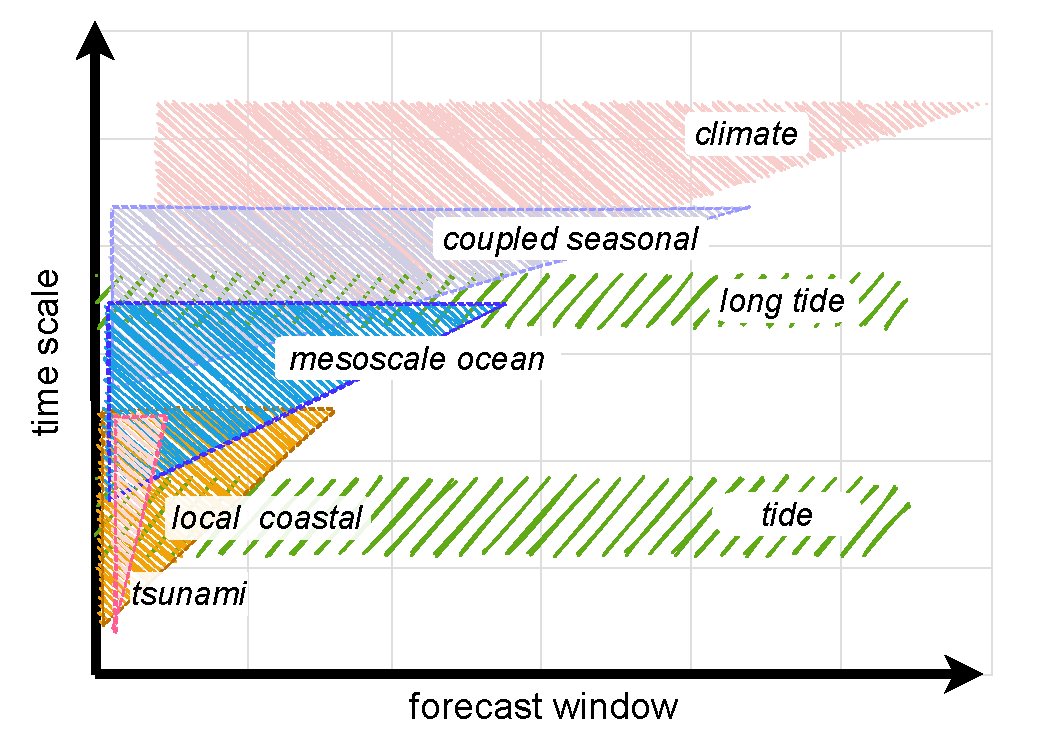
\includegraphics{figures/diagrams/scales.pdf}
  \caption{Schematic on scalew}
  \label{fig:SCALES}
\end{figure}

\begin{figure}[h]\centering
  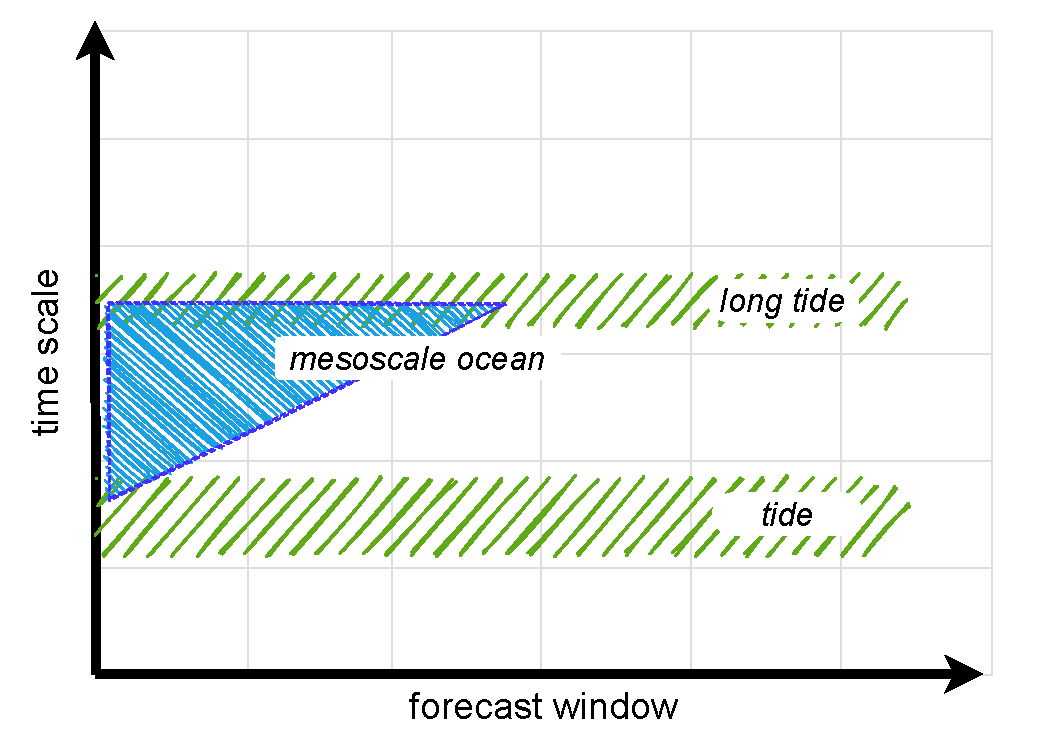
\includegraphics[width=130mm]{figures/diagrams/scales_focus.pdf}
  \caption{Schematic on scalew}
\end{figure}

\begin{figure}[h]\centering
  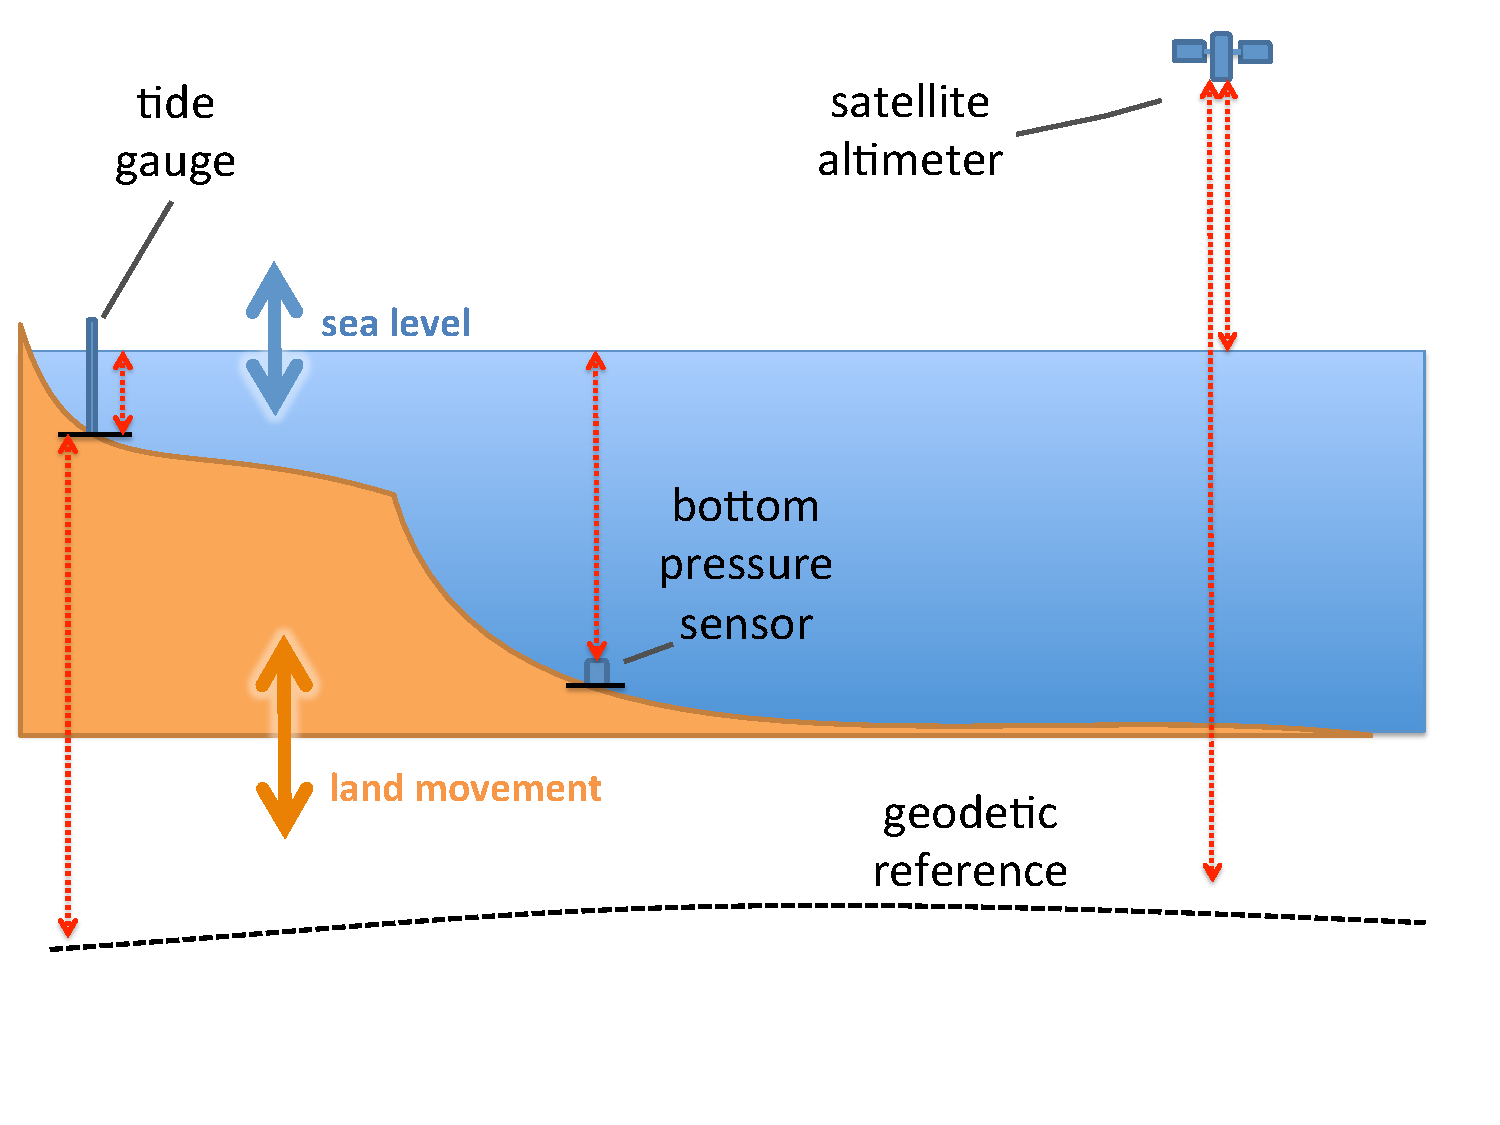
\includegraphics[width=80mm]{figures/diagrams/sealevel_cartoon.pdf}
  \caption{Simplified illustration of the relative nature of sea level and different observing platforms.}
  \label{fig:SEALEVEL}
\end{figure}


\begin{figure}[h]\centering
	\subfloat[Darwin in Northern Australia - large diurnal tide.]{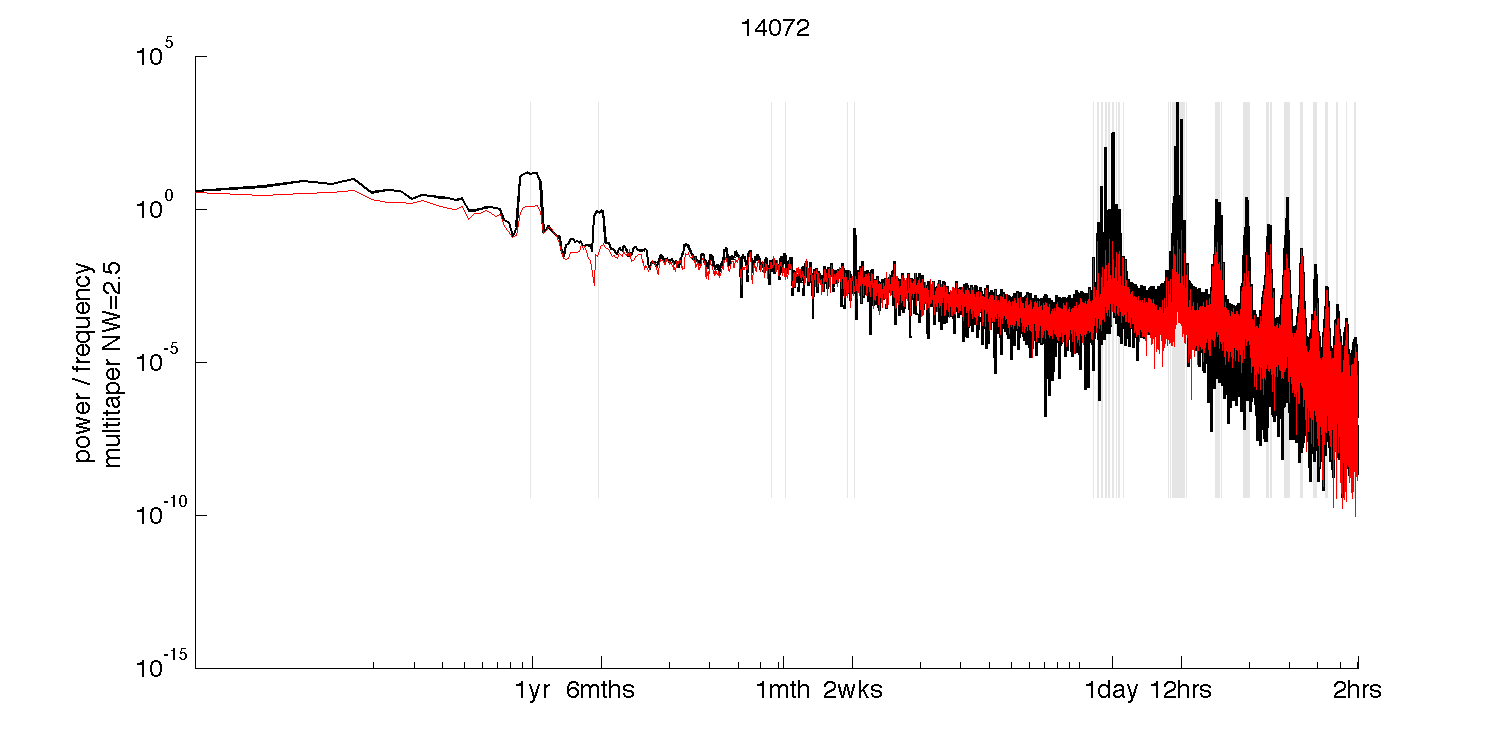
\includegraphics[width=130mm]{figures/plots/plot_14072.png}} \\
	\subfloat[Esperence in Southern Australia - powerful synoptic signal.]{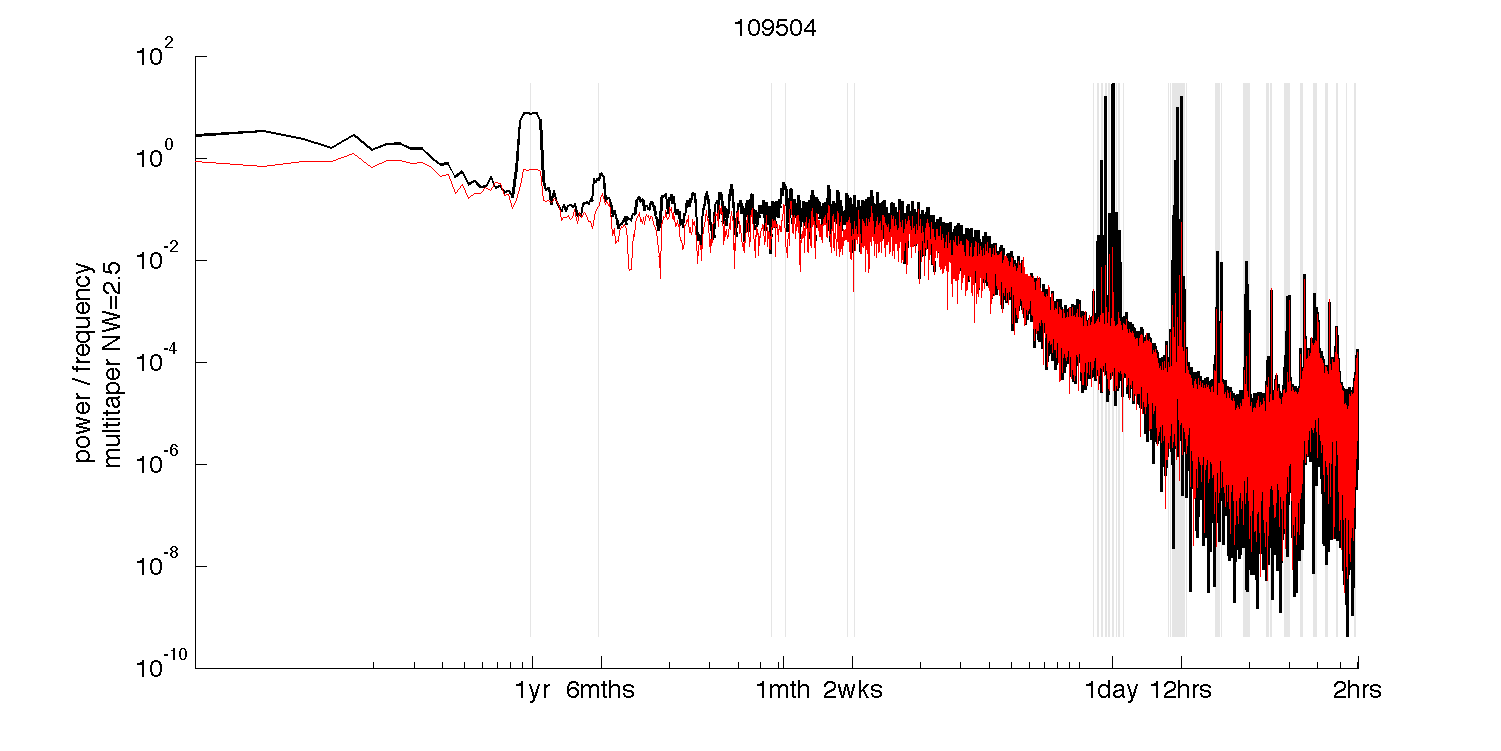
\includegraphics[width=130mm]{figures/plots/plot_109504.png}}
	\caption{Spectral estimates from two coastal tide gauges. Hourly data, black = observations, red = tidal residual. An example of a `mixed spectra' \citep{Percival:1998tw}, in the sense of that discrete spectral lines appear embedded in a background continuum of coloured noise.  The overall `redness' of the spectra and the prominence of spikes at tidal frequencies is highlighted }
    \label{fig:SPECTRA_EG}
\end{figure}

\end{frame}